\documentclass[letter]{article}

\usepackage[spanish,es-nodecimaldot]{babel}
\usepackage[margin=1in]{geometry}
\usepackage{amsmath}
\usepackage{amsthm}
\usepackage{amssymb}
\usepackage[utf8]{inputenc}
\usepackage{graphicx, color}
\usepackage{algorithm}
\usepackage{algpseudocode}
\usepackage{mathrsfs}
% Cambiar el estilo de las listas
\renewcommand{\labelitemi}{$\bullet$}

% Some definitions
\floatname{algorithm}{Algoritmo}

% Author info
\title{Secuencias Mayoritarias}
\author{Alejandro Morales Contreras$^1$}
\date{
	$^1$Departamento de Ingeniería de Sistemas, Pontificia Universidad Javeriana\\Bogotá,  Colombia \\
	\texttt{a.moralesc@javeriana.edu.co}\\~\\
	\today
}

\begin{document}
\maketitle

\tableofcontents

\section{Enunciado del problema} \label{enunciado}

Escriba dos algoritmos para solucionar el problema: ``indicar si una secuencia es mayoritaria y, en caso de serlo, informar el elemento mayoritario". Una secuencia es mayoritaria cuando al menos la mitad de sus elementos tienen el mismo valor, por ejemplo: \par

\[ S = \left< 1, 2, 10, 1, 2, 1, 1, 1, 1, 1, 1, 1, 1, 1, 1, 1, 1, 1, 33, 4, 15, 1, 3, -1, 1, 1, 1, 1, 1 \right> \]

es mayoritaria y el elemento mayoritario es 1. Los dos algoritmos serán: \par

\begin{enumerate}
    \item Iterativo.
    \item Basado en la estrategia ``dividir-y-vencer".
\end{enumerate}

\section{Formalización del problema} \label{formalizacion}

El problema de secuencias mayoritarias se define a partir de:
  \begin{enumerate}
    \item una secuencia $S$ de elementos $a\in \mathbb{T}$,
    \item una relación de igualdad $a=b ~\forall a,b \in S$ y
    \item una relación de orden parcial $a<b ~\forall a,b \in S$
  \end{enumerate}
retornar una pareja $(x, y)$ donde $x$ representa si la secuencia es mayoritaria o no, y $y$ representa el elemento mayoritario. \par

\begin{itemize}
    \item Entradas:
    \begin{itemize}
        \item $S = \left< a_i \in \mathbb{T} \right> ~ | ~ 1\le i \le n \land n \geq 1$.
        \item $a=b \in \mathbb{T} \times \mathbb{T}$, una relación de igualdad.
        \item $a<b \in \mathbb{T} \times \mathbb{T}$, una relación de orden parcial.
    \end{itemize}
    \item Salidas:
    \begin{itemize}
        \item $x 
            \begin{cases}
                1, & \text{if } \exists y \in S ~ | ~ \sum_{i=1}^{n}[S_i=y] > \lfloor |S| \div 2 \rfloor,\\
                0, & \text{else}.
            \end{cases}$
        \item $y \in S \cup \left< 0 \right>$
    \end{itemize}
\end{itemize}

\section{Algoritmos de solución} \label{algoritmos}

\subsection{Iterativo} \label{algoritmos:iterativo}

\subsubsection{Idea general de la solución} \label{algoritmos:iterativo:idea}

Una primera solución ingenua que podría surgir para este problema, sería el de recorrer la secuencia uno a uno, y por cada elemento, volver a recorrer la secuencia para contar cada vez que aparece. Esta solución tendría una complejidad $O(n^2)$, ya que consistiría de dos ciclos anidados. \par

De aquí nace la idea de utilizar una estructura de datos que facilite el conteo de los datos: los mapas. El mapa permitiría recorrer toda la secuencia, e ir contando cuántas veces aparece cada elemento, colocando el elemento como llave y su valor como la cantidad de veces que aparece. Finalmente, solo bastaría recorrer las llaves del mapa y encontrar una que aparezca más de $\lfloor |S| \div 2 \rfloor$ veces. \par

Cabe resaltar que dependiendo de la implementación de mapa que se utilice, la complejidad variaría para las inserciones y búsquedas que se realizan. Un análisis de complejidad más detallado se hace en la sección \ref{algoritmos:iterativo:complejidad}. \par

\subsubsection{Escritura del algoritmo} \label{algoritmos:iterativo:algoritmo}

La solución se presenta en el algoritmo \ref{alg:iterativo} donde:

\begin{itemize}
    \item $\textsc{Exists}(M,k)$ retorna 1 si $k$ es una llave que existe en el mapa $M$ o 0 si no existe
    \item $\textsc{Keys}(M)$ retorna un arreglo con todas las llaves definidas en el mapa $M$
\end{itemize}

\newpage

\begin{algorithm}[!ht]
\caption{Determinar secuencia mayoritaria de forma iterativa.}
\label{alg:iterativo}
\begin{algorithmic}[1] 
\Procedure{IsMajorityIterative}{$S$}
    \State \textbf{let} $M<k,v>$ \textbf{be a map}
    \For{$i \leftarrow 1 ~\mathbf{to}~ |S|$}
        \If{\Call{Exists}{$M, S_i$}}
            \State $M[S_i] \leftarrow M[S_i] + 1$
        \Else
            \State $M[S_i] \leftarrow 1$
        \EndIf
    \EndFor
    \State $K \leftarrow \Call{Keys}{M}$
    \State $i \leftarrow 0$
    \State $is\_majority \leftarrow 0 \land v \leftarrow 0$
    \While{$i < |K| \land is\_majority = 0$}
        \State $i \leftarrow i + 1$
        \If{$M[K_i] > \lfloor |K| \div 2 \rfloor$}
            \State $is\_majority \leftarrow 1$
            \State $v \leftarrow M[K_i]$
        \EndIf
    \EndWhile
    \State \Return $is\_majority, v$
\EndProcedure
\end{algorithmic}
\end{algorithm}

\subsubsection{Análisis de complejidad} \label{algoritmos:iterativo:complejidad}

Como se mencionó anteriormente, la implementación de mapa que se utilice varía la complejidad que se obtiene con esta solución. \par

En C++, se pueden analizar dos implementaciones de mapas que existen en la librería estándar: \textit{map} y \textit{unordered\_map}. El primero está implementado utilizando un árbol roji-negro, y su complejidad de inserción y búsqueda es $O(\log n)$ tanto para el peor de los casos como el promedio. Debido que para la solución implementada, en el peor de los casos todos los elementos se repiten una sola vez y terminarían apareciendo una sola vez en el mapa, se recorrerían todas las llaves disponibles ($|S|$) y se buscarían dentro del mapa cada vez ($\log |S|$). Finalmente, la complejidad sería de $O(|S| \log |S|)$. \par

Para la segunda implementación disponible, se utilizan hash tables, y su complejidad de inserción y búsqueda es $\Theta(1)$ en el caso promedio y $O(n)$ en el peor de los casos. Sin embargo, el peor de los casos suele ocurrir solo cuando se utilizan llaves poco comunes. Siguiendo la misma lógica analizada en el punto anterior, se tendría una complejidad de $\Theta(|S|)$ en el caso promedio y $O(|S|^2)$ en el peor de los casos. \par

En Java, existen dos implementaciones que siguen la misma lógica: \textit{TreeMap} y \textit{HashMap} respectivamente. Por su parte, en Python los diccionarios siguen la misma lógica de los \textit{unordered\_map}. \par

\subsubsection{Invariante} \label{algoritmos:iterativo:invariante}

La invariante es que existen $1 \leq i \leq |S|$ llaves en el mapa, y al menos una de ellas tiene un valor asociado mayor a $\lfloor |S| \div 2 \rfloor$ o la secuencia no es mayoritaria.

\begin{itemize}
    \item Inicio: $\Call{Keys}{M} = \emptyset$
    \item Procesamiento: $M[S_i] 
        \begin{cases}
            M[S_i] + 1, & \text{if } \Call{Exists}{M,S_i} \\
            1, & \text{else }
        \end{cases}$
    \item Fin: $\exists x \in S ~|~ M[x]> \lfloor |S| \div 2 \rfloor \lor x \notin S$
\end{itemize}

\newpage

\subsection{Dividir y vencer} \label{algoritmos:dividir}

\subsubsection{Idea general de la solución} \label{algoritmos:dividir:idea}

Para aplicar la estrategia dividir y vencer, el hecho de que los elementos no traigan algún tipo de relación entre ellos dificulta el proceso de recorrer la secuencia para llegar al problema más sencillo. Sin embargo, una manera fácil de crear esta relación sería ordenando la secuencia con un algún algoritmo de ordenamiento adecuado para tener los elementos iguales seguidos entre sí. \par

Después de ordenados los datos, se puede ver que para que se cumpla la condición de que exista un elemento mayoritario que aparezca al menos $\lfloor |S| \div 2 \rfloor$ veces, este \textbf{necesariamente} debe ubicarse una vez en la posición de la mitad después del ordenamiento. Entonces podemos asumir que: a) la secuencia es mayoritaria y b) que el elemento que se ubique en la mitad de la secuencia es el elemento mayoritario. Ahora solo basta probar que el elemento mayoritario aparece más de la mitad de veces. Si esto no se cumple, la secuencia no es mayoritaria. \par

Podemos representar esta situación en la figura \ref{fig:secuencia_inicial}, en donde tenemos una secuencia S de tamaño $|S|=13$ con punto medio en el índice $7$. Decimos entonces que este elemento $e$ es el mayoritario y los otros dentro de la secuencia los podemos marcar con $X$ ya que no son relevantes si no son iguales a $e$.

\begin{figure}[!ht]
\centering
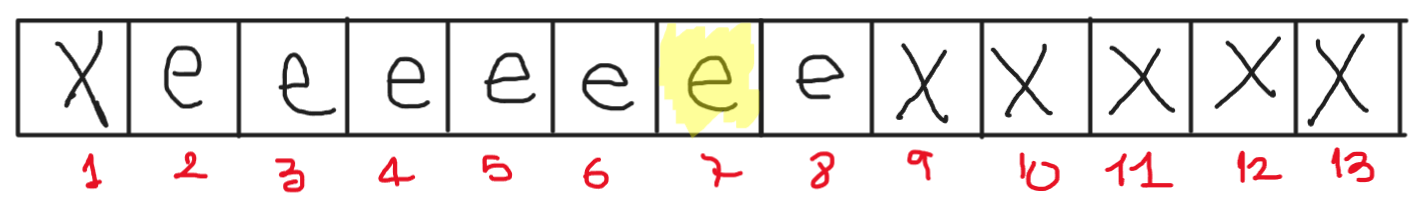
\includegraphics[scale=0.2]{img/fig1.png}
\vspace{-1em}
\caption{Secuencia inicial}
\label{fig:secuencia_inicial}
\end{figure}

El proceso consiste ahora en hacer una especie de búsqueda binaria hacia la izquierda y derecha de este primer pivote, con el fin de determinar en qué posición se encuentran el primer y último elemento mayoritario. Después de conocer esto, solo basta restar estas posiciones para saber cuántos de estos elementos hay. \par

Para hacer la búsqueda, determinamos el inicio y fin de la sub-secuencia, calculamos el pivote y damos un salto hacia este. Parados en este, determinamos si es o no el elemento mayoritario (equivalencia). Si lo es, nos seguimos moviendo en esa dirección. Sin embargo, si no, debemos movernos en dirección contraria porque nos pasamos. El algoritmo acaba cuando el inicio y el fin es el mismo elemento, que sería la posición del primer (o último) elemento mayoritario. \par

Un ejemplo de búsqueda se presenta en la figura \ref{fig:busqueda}. 

\begin{figure}[!ht]
\centering
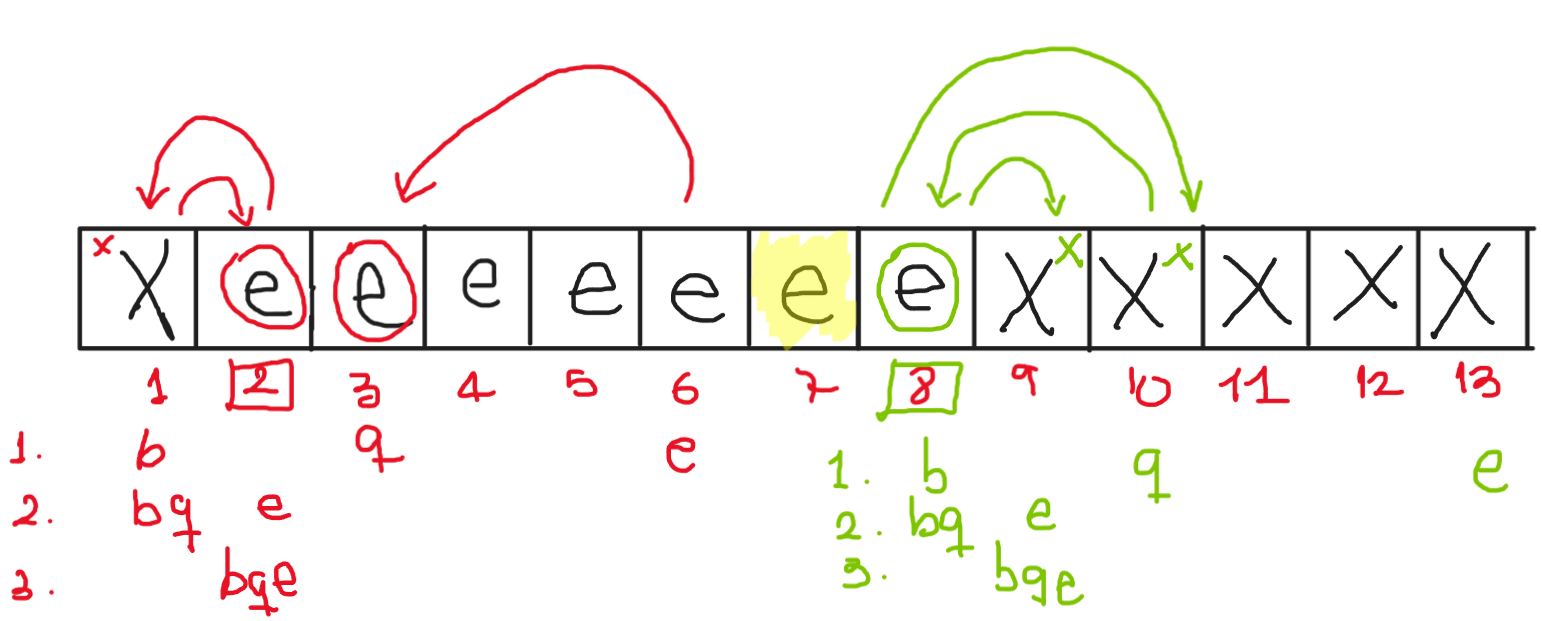
\includegraphics[scale=0.2]{img/fig2.png}
\vspace{-1em}
\caption{Proceso de búsqueda}
\label{fig:busqueda}
\end{figure}

Hacia la izquierda, el primer pivote es $(1+6)/2=3$ y como en esta posición está el elemento mayoritario, seguimos hacia la izquierda. El segundo pivote es $(1+2)/2=1$ y como en esta posición no está el elemento mayoritario, cambiamos hacia la derecha. El tercer pivote es $(2+2)/2=2$ y en esta posición está el elemento mayoritario.Como en esta posición el inicio y fin es el mismo, hemos acabado. La última posición conocida del elemento mayoritario fue el índice $2$. \par

Hacia la derecha, el primer pivote es $(8+13)/2=10$ y como en esta posición no está el elemento mayoritario, vamos hacia la izquierda. El segundo pivote es $(8+9)/2=8$ y como en esta posición está el elemento mayoritario, vamos hacia la derecha. El tercer pivote es $(9+9)/2=9$ y en esta posición no está el elemento. Como en esta posición el inicio y el fin es el mismo, hemos acabado. La última posición conocida del elemento mayoritario fue el índice $8$. \par

Finalmente, se hace la operación $8-2+1$ y se determina que el elemento aparece $7$ veces. Como $7$ es mayor que $|S| \div 2$, entonces la secuencia es mayoritaria y el elemento mayoritario es $e$. \par

\subsubsection{Escritura del algoritmo} \label{algoritmos:dividir:algoritmo}

Donde:

\begin{itemize}
    \item $\Call{Sort}{S}$ es un algoritmo que ordena la secuencia
\end{itemize}

\begin{algorithm}[!ht]
\caption{Determinar secuencia mayoritaria de forma dividir y vencer.}
\label{alg:dividir}
\begin{algorithmic}[1] 
\Procedure{IsMajorityDivideAndConquer}{$S$}
    \State \Call{Sort}{$S$} 
    \State $v \leftarrow S_{\lfloor (|S|+1) \div 2 \rfloor}$
    \State $i \leftarrow \Call{FindMajorityLimit}{S,v,1,\lfloor (|S|+1) \div 2 \rfloor-1,-1,\lfloor |S| \div 2 \rfloor}$
    \State $j \leftarrow \Call{FindMajorityLimit}{S,v,\lfloor (|S|+1) \div 2 \rfloor+1,|S|,1,\lfloor |S| \div 2 \rfloor}$
    \State $count \leftarrow j-i+1$
    \State $is\_majority \leftarrow 1$
    \If{$count \leq \lfloor |S| \div 2 \rfloor$}
        \State $is\_majority \leftarrow 0$
        \State $v \leftarrow 0$
    \EndIf
    \State \Return $is\_majority, v$
\EndProcedure
\end{algorithmic}
\end{algorithm}

\begin{algorithm}[!ht]
\caption{Encontrar posición límite del elemento mayoritario.}
\label{alg:encontrar}
\begin{algorithmic}[1] 
\Procedure{FindMajorityLimit}{$S,value,b,e,dir,last$}
    \If{b=e}
        \If{$S_q = value$}\
            \State $last \leftarrow b$
        \EndIf
        \State \Return $last$
    \Else
        \State $q \leftarrow \lfloor (b+e) \div 2 \rfloor$
        \If{$S_q = value$}
            \If{$dir = 1$}
                \State \Return \Call{FindMajorityLimit}{$S,value,q+1,e,dir,q$}
            \Else
                \State \Return \Call{FindMajorityLimit}{$S,value,b,q-1,dir,q$}
            \EndIf
        \Else
            \If{$dir = 1$}
                \State \Return \Call{FindMajorityLimit}{$S,value,b,q-1,dir,last$}
            \Else
                \State \Return \Call{FindMajorityLimit}{$S,value,q+1,e,dir,last$}
            \EndIf
        \EndIf
    \EndIf
\EndProcedure
\end{algorithmic}
\end{algorithm}

\subsubsection{Análisis de complejidad} \label{algoritmos:dividir:complejidad}

El algoritmo de solución consite en dos partes imporantes: el ordenamiento de la secuencia y la búsqueda de los límites, $O=O_1+O_2$, en donde solo se preserva la de mayor complejidad. La complejidad del ordenamiento está dada por el algoritmo escogido para la secuencia, entonces $O(\Call{Sort}{|S|}$. \par

Por su parte, la búsqueda de los límites es un algoritmo dividir y vencer, y su complejidad puede ser expresada así y hallada a través del teorema maestro: \par

\[ T(n) = T(\frac{n}{2}) + O(1) \]

Utilizando las tres ecuaciones, se encuentra:

\begin{enumerate}
    \item $1 = n^{\log_b(a-\epsilon)} = n^{\log_2(1-\epsilon)} \land \epsilon = 0$
    \item $1 = n^{\log_ba} \log_2^kn = n^{\log_21} \log_2^kn \land k = 0 \rightarrow O(n^{\log_21} \log_2^{k+1}n) = O(\log_2n)$
    \item $1 = n^{\log_b(a-\epsilon)} = n^{\log_2(1+\epsilon)} \land \epsilon = 0$
\end{enumerate}

Por ende la complejidad de la búsqueda de los límites es $O(\log |S|)$. Debido a que $O(\Call{Sort}{|S|} > O(\log |S|)$ siempre, incluso para la cota inferior del ordenamiento, la complejidad dependará únicamente de la complejidad del algoritmo de ordenamiento escogido.

\subsubsection{Invariante} \label{algoritmos:dividir:invariante}

La invariante es que después del ordenamiento, el elemento mayoritario existe una vez en la posición de la mitad y en las posiciones $i,j ~|~ i,j \in [1,|S|] \land j-i+1> \lfloor |S| \div 2 \rfloor$ o la secuencia no es mayoritaria.

\end{document}
